\section{Reconstruction of the photon energy}

As the photon is massless, in the production vertex, an electron and a positron
from $\gamma \to e^+e^-$ have their momenta parallel to each other.
In that point, the photon energy can be approximated as
\begin{equation} \label{eq:egamma}
  E_\gamma = P(e^+) + P(e^-) 
\end{equation}
               
XY views of two typical events are presented in Figure~\ref{figure:rpc07b0s51r0100_xy_view},
Despite $e^+e^-$ pairs are produced several meters upstream of the tracker,
the multiple scattering is small and trajectories of the two particles
in the tracker look like two tangent circles. Because of that, an approximation of \ref{eq:egamma}
should hold rather well, and it will be used in this note.

\begin{figure}[H]
  \begin{tikzpicture}
    \node[anchor=south west,inner sep=0] at (0,0.) {
      % \node[shift={(0 cm,0.cm)},inner sep=0,rotate={90}] at (0,0) {}
      \makebox[\textwidth][c] {
        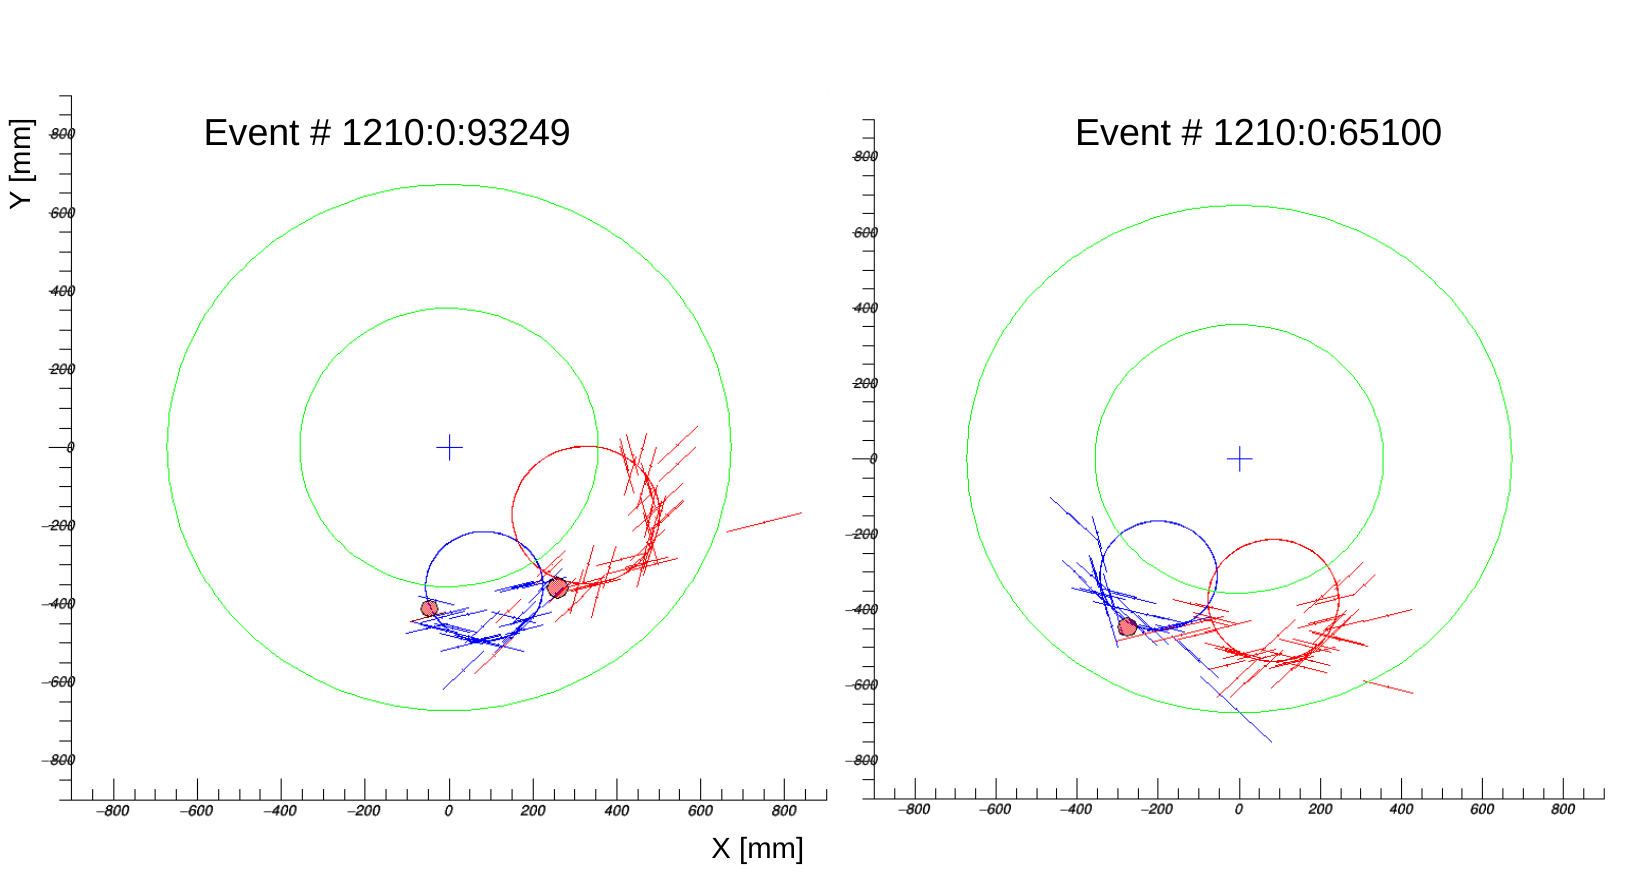
\includegraphics[width=0.9\textwidth]{png/rpc07b0s51r0100_event_display_xy_reconstructed}
      }
    };
    % \node [text width=8cm, scale=1.0] at (14.5,0.5) {$\mu_B$, expected background mean};
    % \node [text width=8cm, scale=1.0, rotate={90}] at (1.5,7.5) { $S_{D}$, ``discovery'' signal strength  };
  \end{tikzpicture}
  \caption{
    \label{figure:rpc07b0s51r0100_xy_view}
    XY tracker view of $\gamma \to e^+e^-$ events
  }
\end{figure}

%%%%%%%%%%%%%%%%%%%%%%%%%%%%%%%%%%%%%%%%%%%%%%%%%%%%%%%%%%%%%%%%%%%%%%%%%%%%%%
\subsection{Converter thickness}

The converter is simulated as a thin gold foil. To choose an optimal thickness ,
we considered three different opetions: 1mm-thick converter, 200 um - and 100 um -thick foils.
Shown in Figure~\ref{figure:sum_mom_vd13}(left) are the distributions of $E_{gamma}^{VD13} = P(e^+)^{VD13} + P(e^-)^{VD13}$,
the sum of MC momenta of an electron and a positron plotted for events with

\begin{itemize}
\item
  an electron an a positron producing N>=20 straw hits in the tracker each
\item
  minimal, out of the two, particle momentum at VD13 P > 30 MeV/c
\end{itemize}

\begin{figure}[H]
  \begin{tikzpicture}
    \node[anchor=south west,inner sep=0] at (0,0.) {
      % \node[shift={(0 cm,0.cm)},inner sep=0,rotate={90}] at (0,0) {}
      % \makebox[\textwidth][c] {
        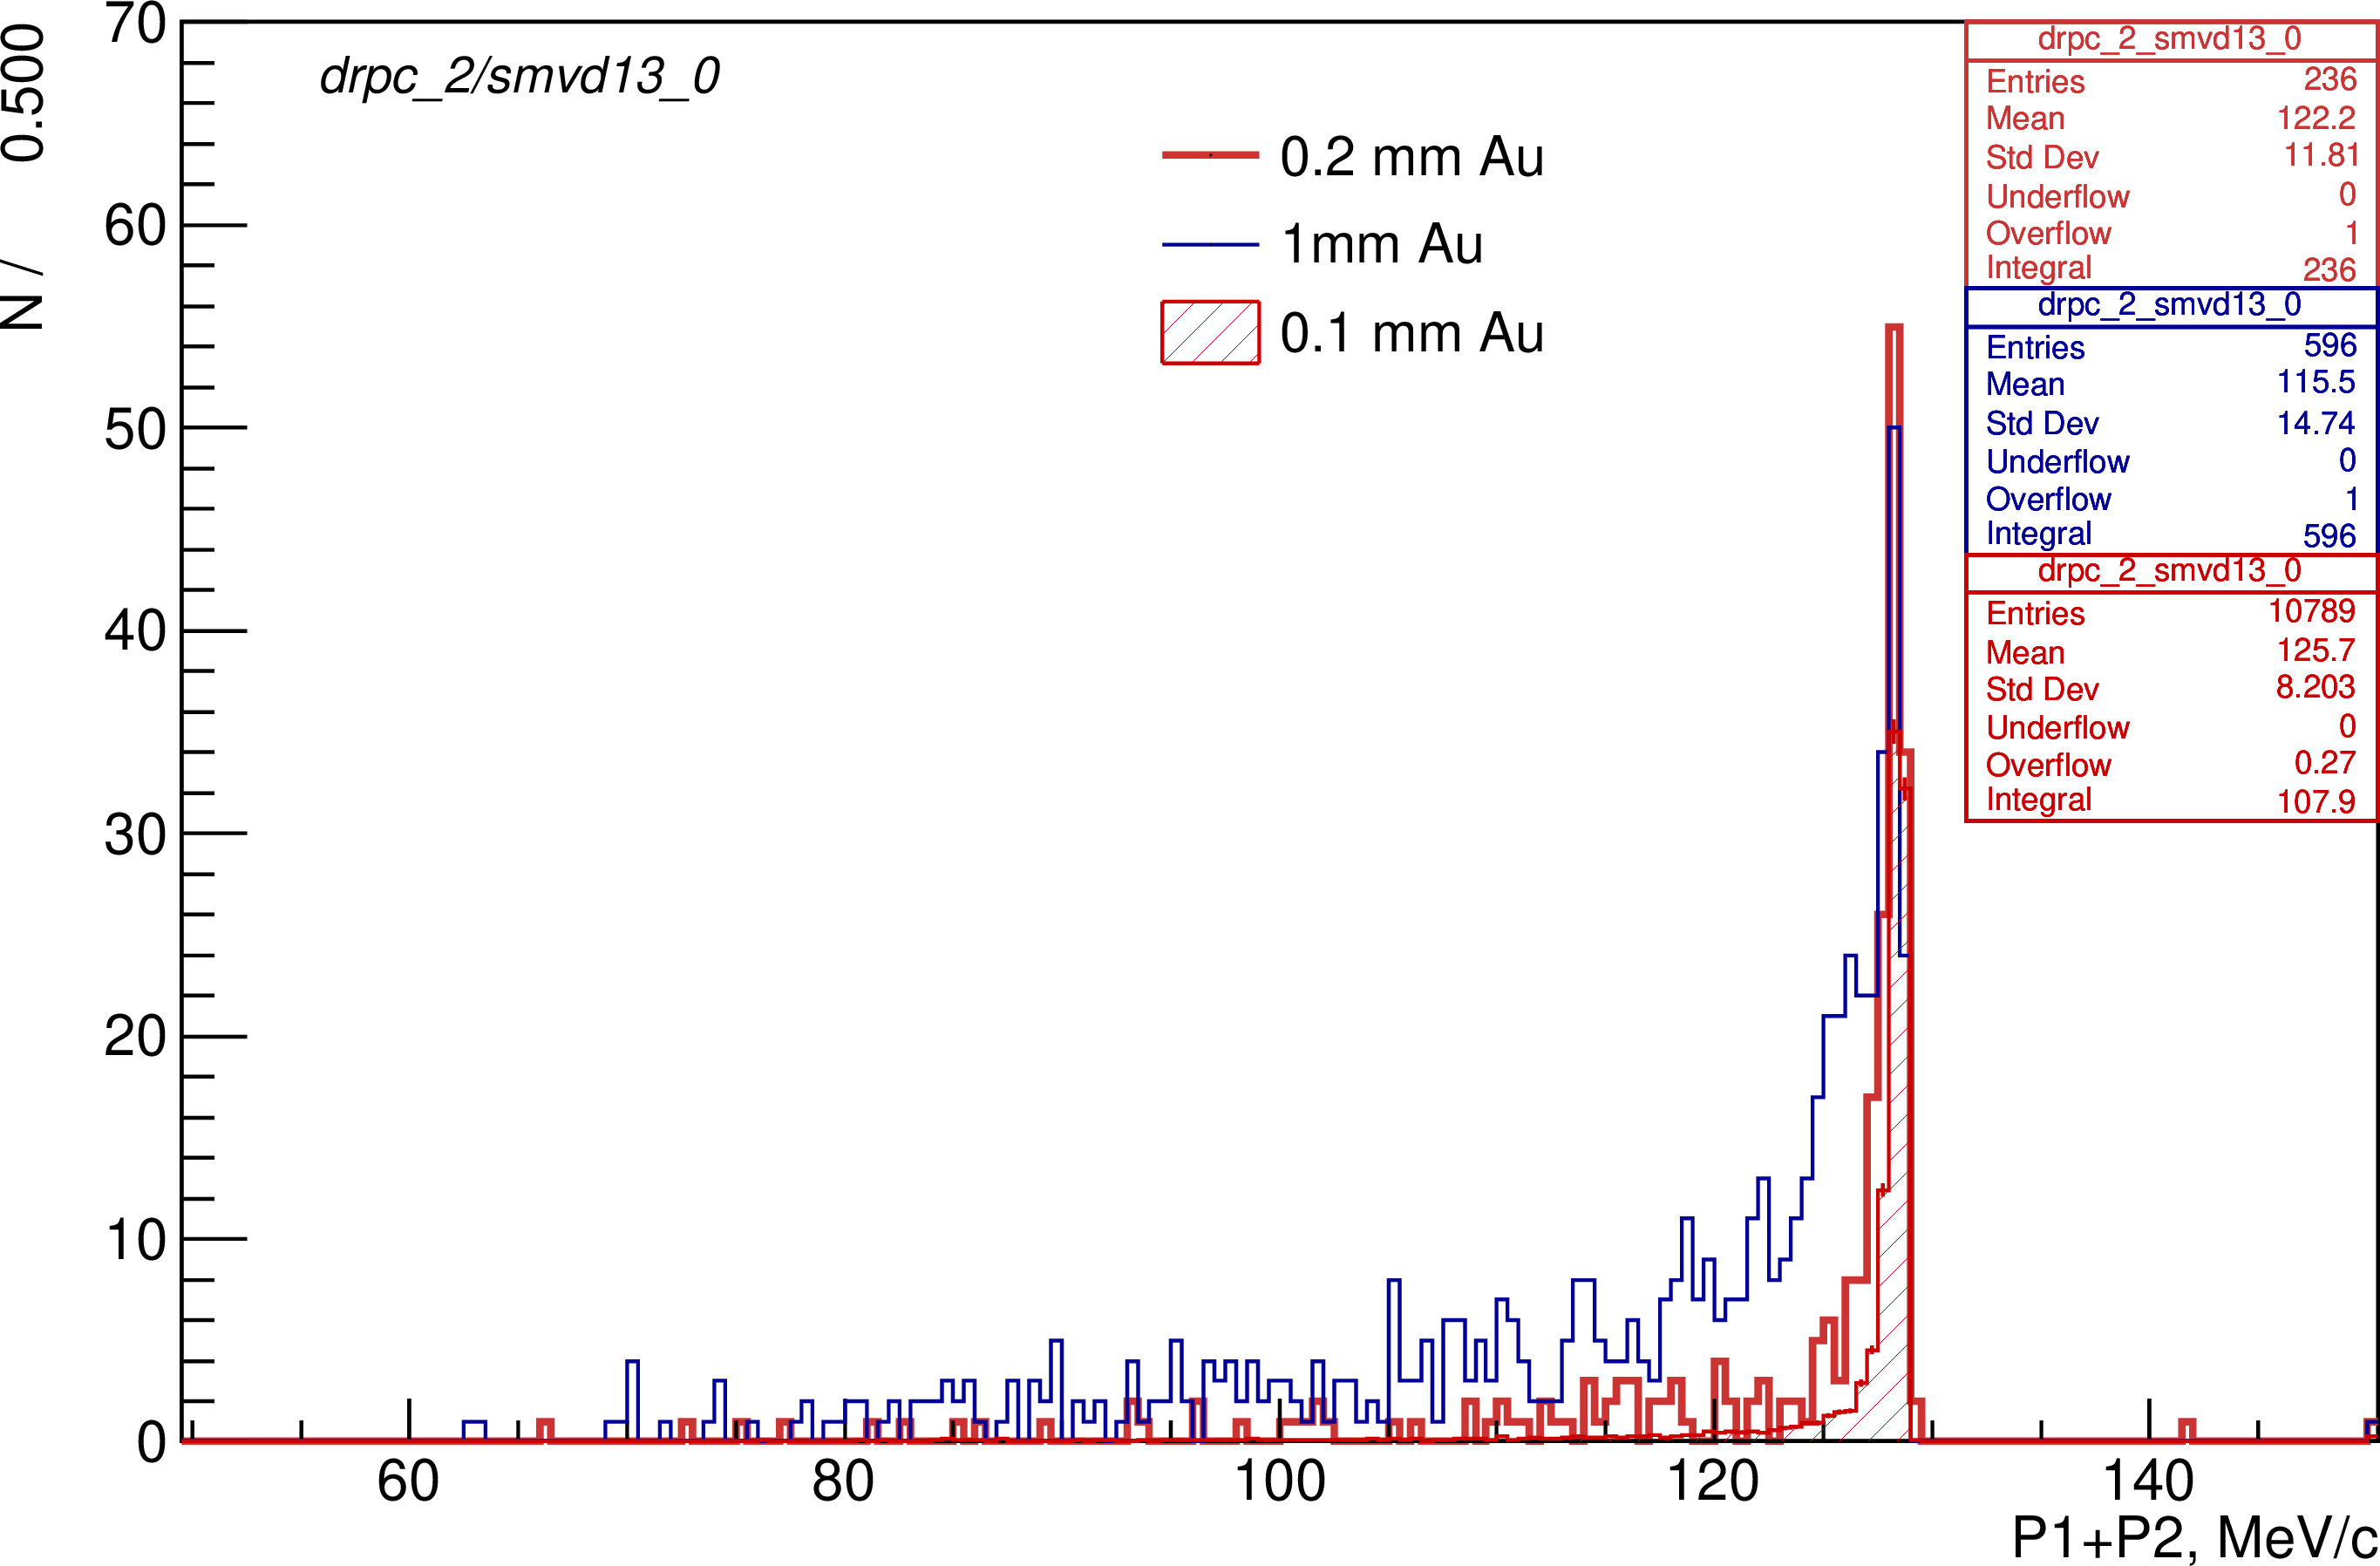
\includegraphics[width=0.54\textwidth]{pdf/figure_00013}
      % }
    };
    \node[anchor=south west,inner sep=0] at (10,0.) {
      % \node[shift={(0 cm,0.cm)},inner sep=0,rotate={90}] at (0,0) {}
      % \makebox[\textwidth][c] {
        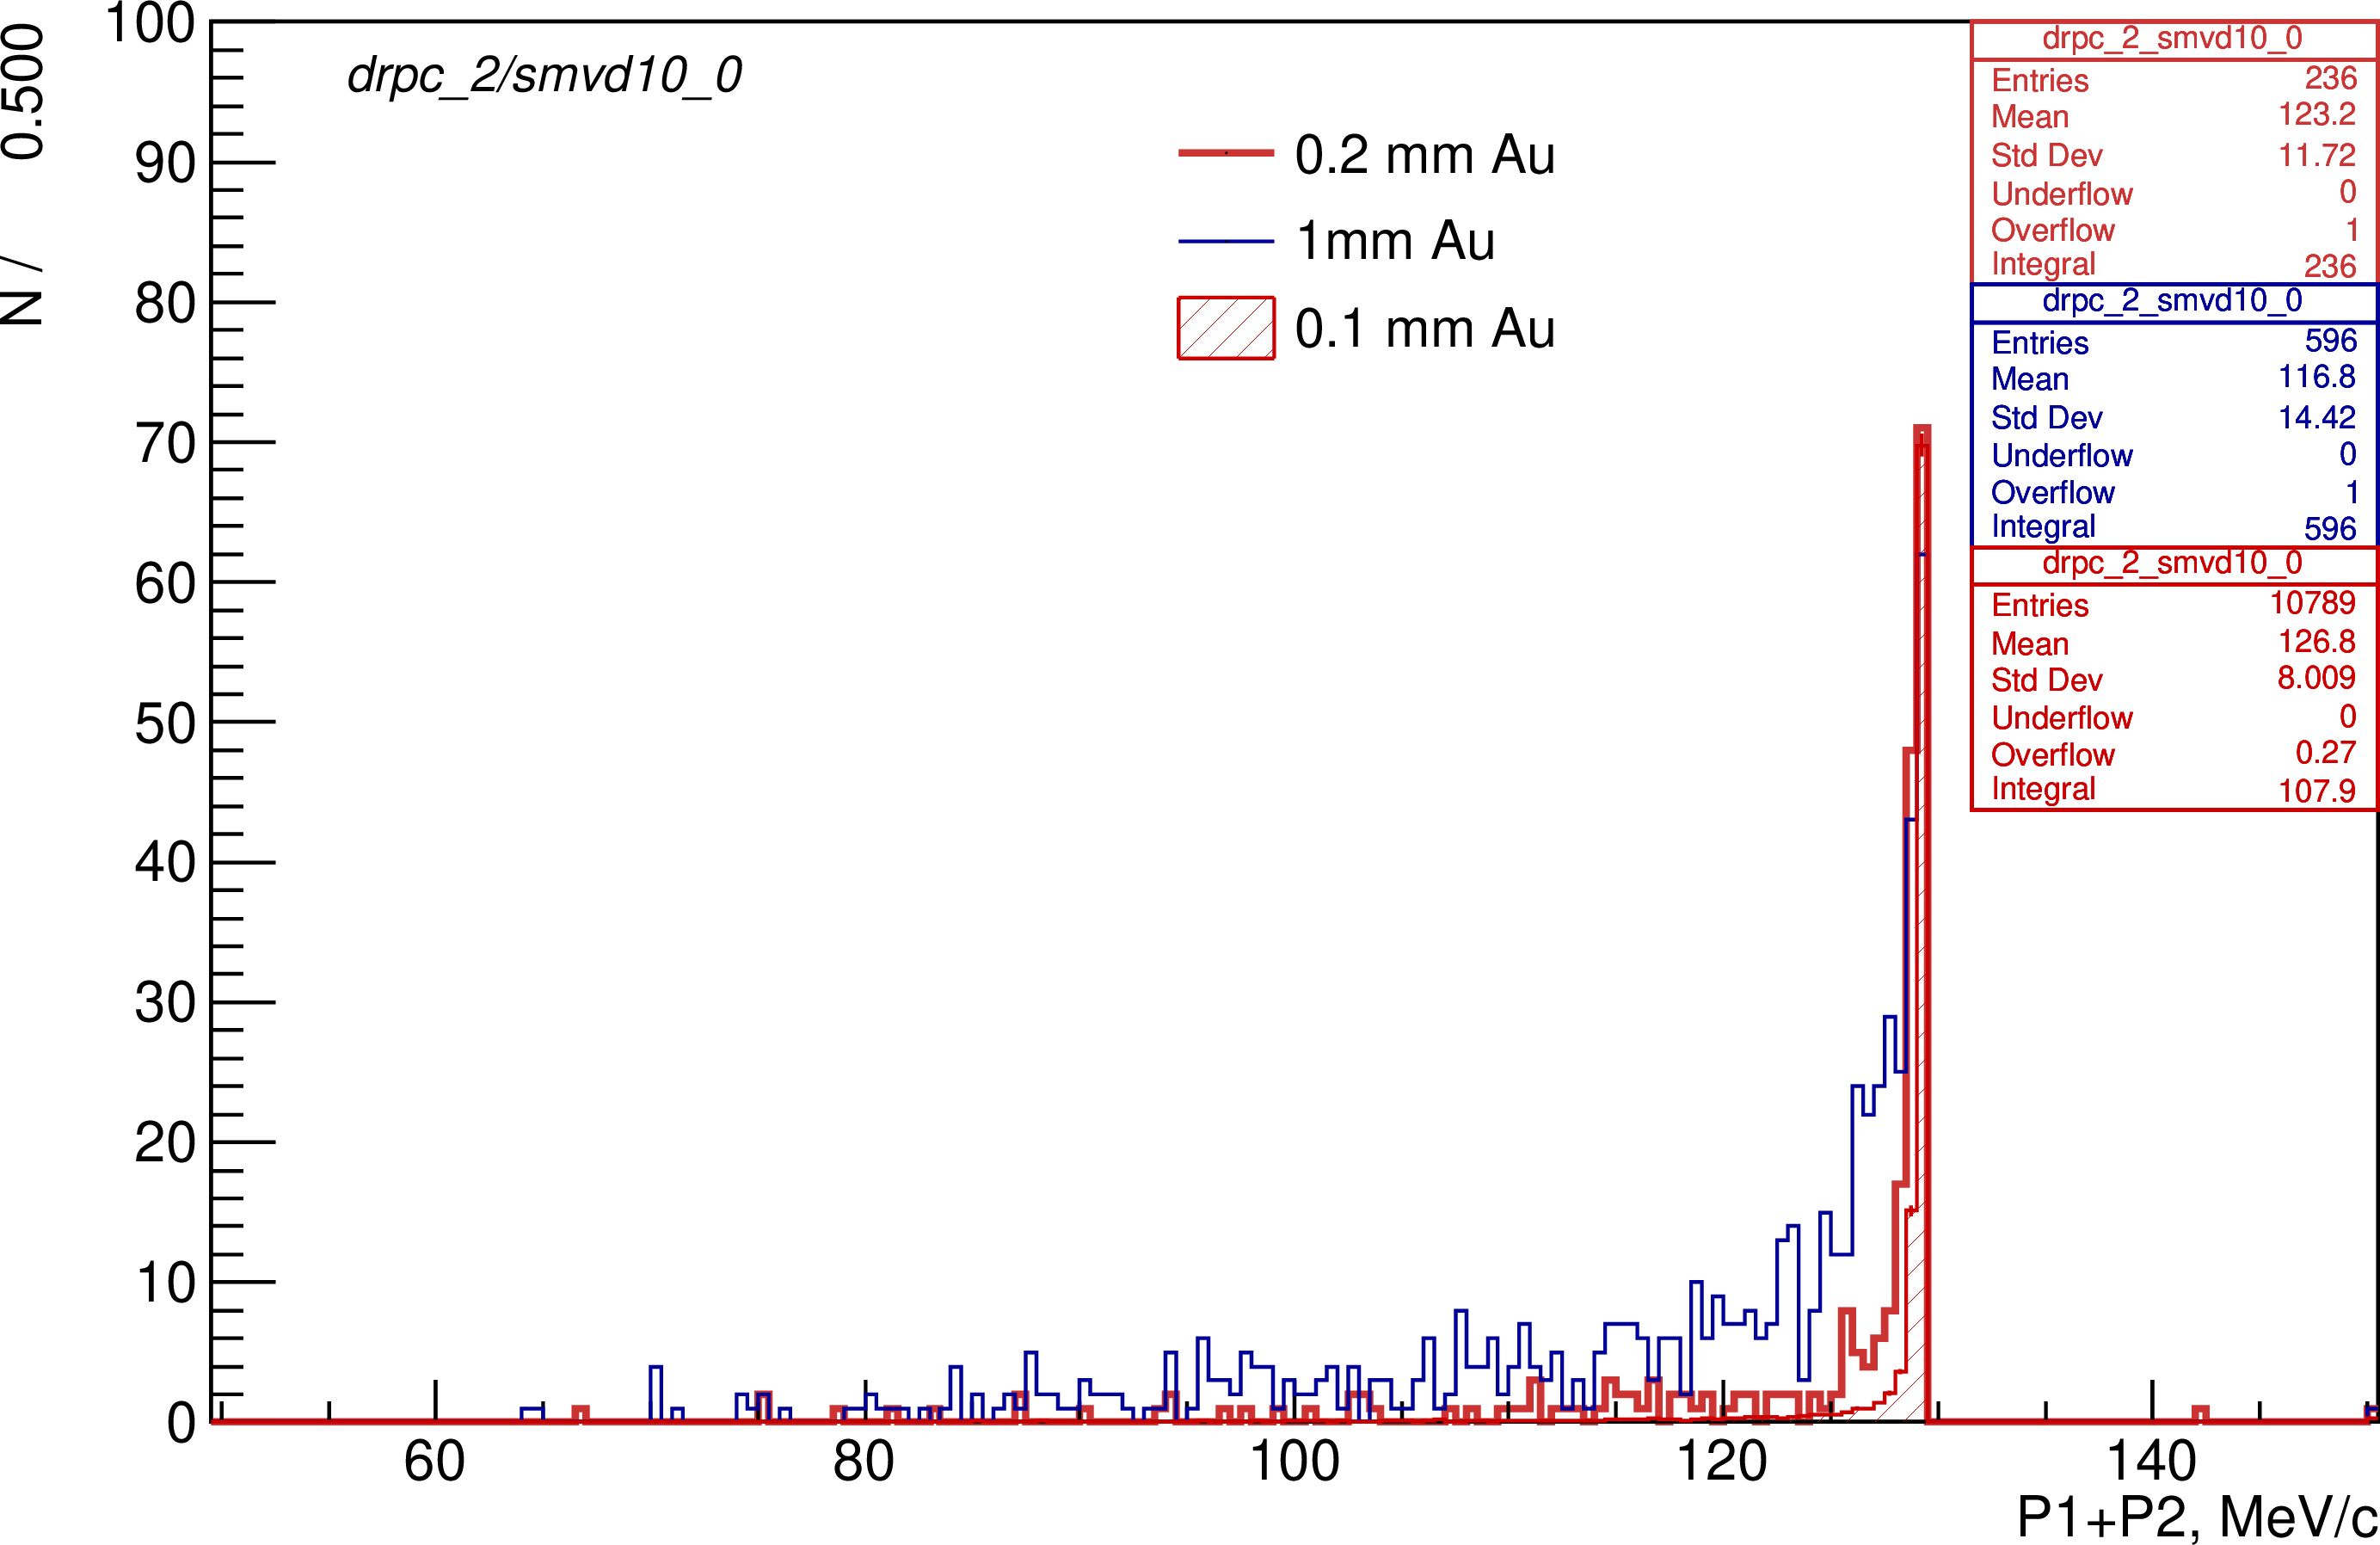
\includegraphics[width=0.54\textwidth]{pdf/figure_00010}
      % }
    };
    % \node [text width=8cm, scale=1.0] at (14.5,0.5) {$\mu_B$, expected background mean};
    % \node [text width=8cm, scale=1.0, rotate={90}] at (1.5,7.5) { $S_{D}$, ``discovery'' signal strength  };
  \end{tikzpicture}
  \caption{
    \label{figure:sum_mom_vd13}
    left: $E_\gamma^{VD13}$ for 1mm, 200 um, and 100-um thick Au converters at R=25 cm ; \\
    right: distributions of $E_\gamma^{VD10}$ for 1mm, 200 um, and 100-um thick Au converters at R=25 cm
  }
\end{figure}

From the left distribution, it becomes clear that while the increasing thickness of the converter improves the
overall event yield, it is the thinnest out of the three considered converter options which produces
more $\gamma \to e^+e^-$ events in the few highest energy bins than thicker converters.

Comparison of the left and right plots in Figure~\ref{figure:sum_mom_vd13} shows the scale of energy
losses in the IPA and in the converter ring itself.

\begin{figure}[H]
  \begin{tikzpicture}
    \node[anchor=south west,inner sep=0] at (0,0.) {
      % \node[shift={(0 cm,0.cm)},inner sep=0,rotate={90}] at (0,0) {}
      \makebox[\textwidth][c] {
        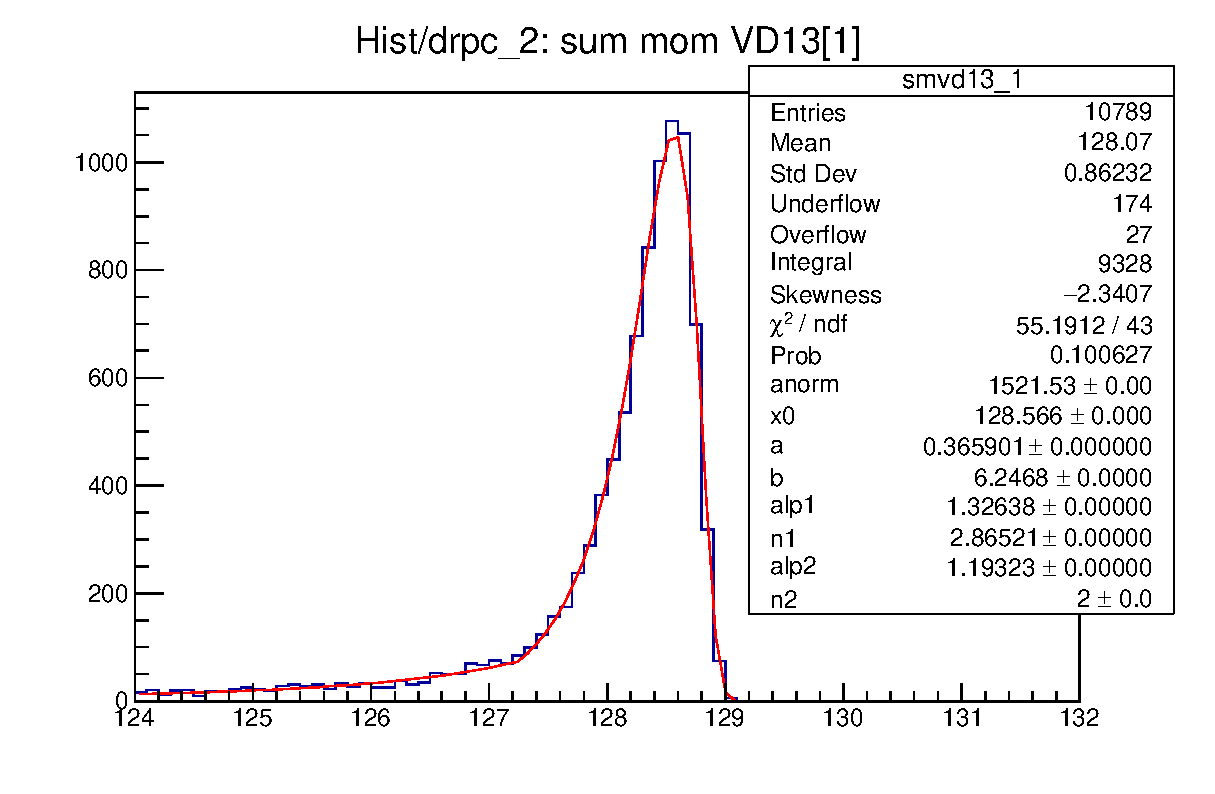
\includegraphics[width=0.9\textwidth]{pdf/figure_00083}
      }
    };
    % \node [text width=8cm, scale=1.0] at (14.5,0.5) {$\mu_B$, expected background mean};
    % \node [text width=8cm, scale=1.0, rotate={90}] at (1.5,7.5) { $S_{D}$, ``discovery'' signal strength  };
  \end{tikzpicture}
  \caption{
    \label{figure:00083}
    fit of the $E_\gamma^{VD13}$ distribution with the SU2020 resolution function defined by
    the Eq.\ref{eq:dio_mom_res}.
    The mean energy loss of two particles traveling from the converter to the tracker is about 0.8 MeV,
    the contribution of struggling to the energy resolution is $\sim 0.7$ MeV/c FWHM. \\
    The fit uncertainty on x0, parameter corresponding to the maximum of the spectrum,
    is less than 1 keV.
  }
\end{figure}

Figure ~\ref{figure:00083} shows the distribution of $E_\gamma^{VD13}$
for 100 um converter with the binning of 100 keV/c and its fit with the resolution function introduced
in the SU2020 paper \cite{MU2E_SU2020_PAPER}:

\begin{equation}
  \label{eq:dio_mom_res}
  R(x) =
 \begin{cases}
    A_1 \cdot (B_1-x)^{-N_1}                                 & x < -\alpha_1 \\
    A_0 \cdot \exp (a_0 \cdot (b_0 \cdot x - e^{b_0 \cdot x})) & -\alpha_1< x < \alpha_2 \\
    A_2 \cdot (B_2+x)^{-N_2}                                 &  x > \alpha_2
  \end{cases}.
\end{equation}
, where $x = p-p_0$, and $p_0$ is the position of the distribution maximum.
The most probable energy loss is about 800 keV/c, 
and the resolution function has the FWHM of about 700 keV/c.
These numbers are not very different from the corresponding numbers for conversion electrons.

%%% Local Variables:
%%% mode: latex
%%% TeX-master: t
%%% End:
